%%%%%%%%%%%%%%%%%%%%%%%%%%%%%%%%%%%%%%%%%
% Beamer Presentation
% LaTeX Template
% Version 1.0 (10/11/12)
%
% This template has been downloaded from:
% http://www.LaTeXTemplates.com
%
% License:
% CC BY-NC-SA 3.0 (http://creativecommons.org/licenses/by-nc-sa/3.0/)
%
%%%%%%%%%%%%%%%%%%%%%%%%%%%%%%%%%%%%%%%%%

%----------------------------------------------------------------------------------------
%	PACKAGES AND THEMES
%----------------------------------------------------------------------------------------

\documentclass[UTF8,aspectratio=169,14pt]{ctexbeamer}

\usepackage{hyperref}
\hypersetup{
	colorlinks=true,
	linkcolor=red,
	anchorcolor=blue,
	citecolor=green
}

\mode<presentation> {
	
	% The Beamer class comes with a number of default slide themes
	% which change the colors and layouts of slides. Below this is a list
	% of all the themes, uncomment each in turn to see what they look like.
	
	%\usetheme{default}
	%\usetheme{AnnArbor}
	%\usetheme{Antibes}
	%\usetheme{Bergen}
	%\usetheme{Berkeley}
	%\usetheme{Berlin}
	%\usetheme{Boadilla}
	%\usetheme{CambridgeUS}
	%\usetheme{Copenhagen}
	%\usetheme{Darmstadt}
	%\usetheme{Dresden}
	%\usetheme{Frankfurt}
	%\usetheme{Goettingen}
	%\usetheme{Hannover}
	%\usetheme{Ilmenau}
	%\usetheme{JuanLesPins}
	%\usetheme{Luebeck}
	\usetheme{Madrid}
	%\usetheme{Malmoe}
	%\usetheme{Marburg}
	%\usetheme{Montpellier}
	%\usetheme{PaloAlto}
	%\usetheme{Pittsburgh}
	%\usetheme{Rochester}
	%\usetheme{Singapore}
	%\usetheme{Szeged}
	%\usetheme{Warsaw}
	
	% As well as themes, the Beamer class has a number of color themes
	% for any slide theme. Uncomment each of these in turn to see how it
	% changes the colors of your current slide theme.
	
	%\usecolortheme{albatross}
	%\usecolortheme{beaver}
	%\usecolortheme{beetle}
	%\usecolortheme{crane}
	%\usecolortheme{dolphin}
	%\usecolortheme{dove}
	%\usecolortheme{fly}
	%\usecolortheme{lily}
	%\usecolortheme{orchid}
	%\usecolortheme{rose}
	%\usecolortheme{seagull}
	%\usecolortheme{seahorse}
	%\usecolortheme{whale}
	%\usecolortheme{wolverine}
	
	%\setbeamertemplate{footline} % To remove the footer line in all slides uncomment this line
	%\setbeamertemplate{footline}[page number] % To replace the footer line in all slides with a simple slide count uncomment this line
	
	%\setbeamertemplate{navigation symbols}{} % To remove the navigation symbols from the bottom of all slides uncomment this line
}

\usepackage{graphicx} % Allows including images
\graphicspath{{./figs/}}
\usepackage{booktabs} % Allows the use of \toprule, \midrule and \bottomrule in tables
\usepackage{longtable}
\usepackage{listings}
\usepackage{xcolor}
\lstset{numbers=left, %设置行号位置
	numberstyle=\tiny, %设置行号大小
	keywordstyle=\color{blue}, %设置关键字颜色
	commentstyle=\color[cmyk]{1,0,1,0}, %设置注释颜色
	frame=single, %设置边框格式
	escapeinside=``, %逃逸字符(1左面的键),用于显示中文
	%breaklines, %自动折行
	extendedchars=false, %解决代码跨页时,章节标题,页眉等汉字不显示的问题
	xleftmargin=2em,xrightmargin=2em, aboveskip=1em, %设置边距
	tabsize=4, %设置tab空格数
	showspaces=false %不显示空格
}
% Fonts
% \usepackage{libertine}
% \setmonofont{Courier}
\setCJKsansfont[ItalicFont=Noto Serif CJK SC Black, BoldFont=Noto Sans CJK SC Black]{Noto Sans CJK SC}


%----------------------------------------------------------------------------------------
% TITLE PAGE
%----------------------------------------------------------------------------------------

\title[第21讲]{第二十一讲 :异步编程(Asynchronous Programming)} % The short title appears at the bottom of every slide, the full title is only on the title page
\subtitle{第3节:Generators and async/await}
\author{向勇、陈渝、李国良} % Your name
\institute[清华大学] % Your institution as it will appear on the bottom of every slide, may be shorthand to save space
{
  清华大学计算机系 \\ % Your institution for the title page
  \medskip
  \textit{xyong,yuchen,liguoliang@tsinghua.edu.cn} % Your email address
}
\date{\today} % Date, can be changed to a custom date

\begin{document}

\begin{frame}
\titlepage % Print the title page as the first slide
\end{frame}

%----------------------------------------------
\begin{frame}
\frametitle{提纲} % Table of contents slide, comment this block out to remove it
\tableofcontents % Throughout your presentation, if you choose to use \section{} and \subsection{} commands, these will automatically be printed on this slide as an overview of your presentation
% itemize
Ref:
    \begin{itemize}
        \item \href{https://cfsamson.github.io/books-futures-explained/}{Futures Explained in 200 Lines of Rust}
        \item Writing an OS in Rust - \href{https://os.phil-opp.com/async-await/}{Async/Await}
        \item \href{https://zhuanlan.zhihu.com/p/97574385}{零成本异步I/O}
    \end{itemize}

\end{frame}
%----------------------------------------------
% ### ref
% 
% - [Futures Explained in 200 Lines of Rust](https://cfsamson.github.io/books-futures-explained/#futures-explained-in-200-lines-of-rust) [repo at github](https://github.com/cfsamson/books-futures-explained)
% - Writing an OS in Rust - [Async/Await](https://os.phil-opp.com/async-await/)
% - [零成本异步I/O](https://zhuanlan.zhihu.com/p/97574385)
% 
%----------------------------------------------
%%  PRESENTATION SLIDES
%----------------------------------------------
\section{Background} % Sections can be created in order to organize your presentation into discrete blocks, all sections and subsections are automatically printed in the table of contents as an overview of the talk
\section{Futures in Rust} % Sections can be created in order to organize your presentation into discrete blocks, all sections and subsections are automatically printed in the table of contents as an overview of the talk
%----------------------------------------------
%%  PRESENTATION SLIDES
%----------------------------------------------
\section{第3节:Generators and async/await} % Sections can be created in order to organize your presentation into discrete blocks, all sections and subsections are automatically printed in the table of contents as an overview of the talk
\section{Self-Referential Structs \& Pin} % Sections can be created in order to organize your presentation into discrete blocks, all sections and subsections are automatically printed in the table of contents as an overview of the talk
\section{Waker and Reactor} % Sections can be created in order to organize your presentation into discrete blocks, all sections and subsections are automatically printed in the table of contents as an overview of the talk
%----------------------------------------------
\begin{frame}[fragile]
    \frametitle{Concurrency in Rust}
%    \framesubtitle{xxxx}
% ### 21.3 Generators and async/await
% 
% Ref: https://cfsamson.github.io/books-futures-explained/3_generators_async_await.html#generators-and-asyncawait
% 
% #### Concurrency in Rust
% 
% Ref: https://cfsamson.github.io/books-futures-explained/3_generators_async_await.html
% 
    \begin{itemize}
        \item Stackful coroutines (green threads)
        \item Using combinators
        \item Stackless coroutines (generators)
    \end{itemize}
% 
\end{frame}
%----------------------------------------------
\begin{frame}[fragile]
    \frametitle{State Machine Transformation in Future}
%    \framesubtitle{xxxx}
% #### State Machine Transformation in Future
% 
% Ref: https://os.phil-opp.com/async-await/#state-machine-transformation
% https://cfsamson.github.io/books-futures-explained/3_generators_async_await.html#stackless-coroutinesgenerators
% 
%% itemize
    \begin{itemize}
        \item Async in Rust is implemented using {\color{red}Generators}
        \item Generators in Rust are implemented as {\color{red}state machines}
        \item {\color{red}Compiler} transforms the body of the `async` function into a state machine, with each `.await` call representing a different state. \pause
        \item {\color{red}Each state} represents a different pause point of the function
% 
%% figure
    \begin{figure}
    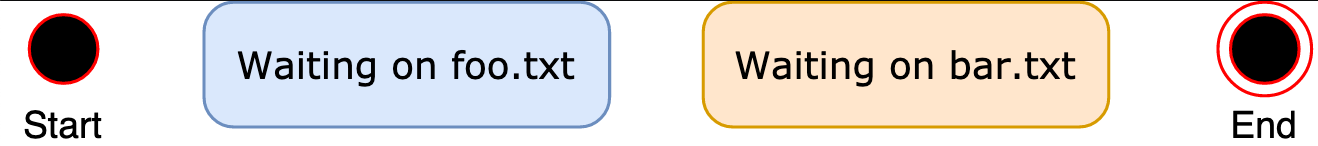
\includegraphics[width=0.4\linewidth]{figs/async-state-machine-states.png}
%    \caption{xxxx}
    \end{figure} \pause
% ![async-state-machine-states](figs/async-state-machine-states.svg)
% 
        \item Arrows represent {\color{red}state switches} and diamond shapes represent alternative ways
% 
%% figure
    \begin{figure}
    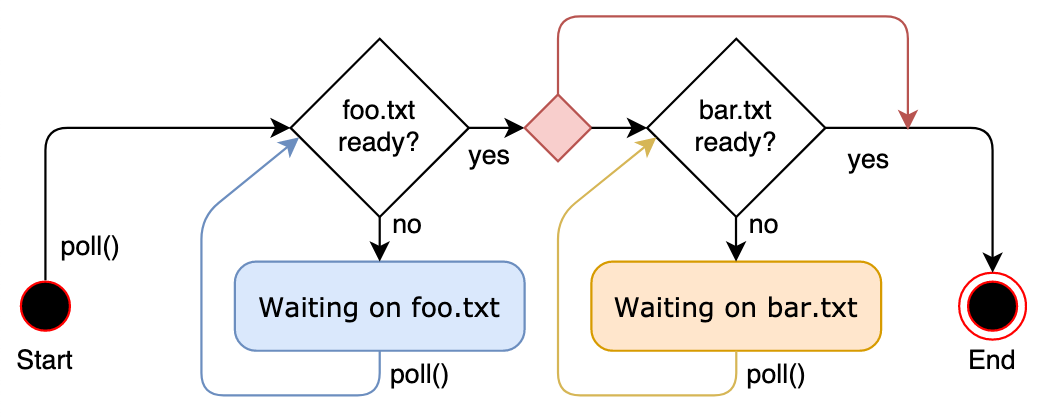
\includegraphics[width=0.55\linewidth]{figs/async-state-machine-basic.png}
%    \caption{xxxx}
    \end{figure}
% ![async-state-machine-basic](figs/async-state-machine-basic.svg)
    \end{itemize}
% 
\end{frame}
%----------------------------------------------
\begin{frame}[fragile]
    \frametitle{State Machine Type: enum ExampleStateMachine}
%    \framesubtitle{xxxx}
% #### State Machine Type
% 
% Ref: https://os.phil-opp.com/async-await/#the-full-state-machine-type
% 
%% itemize
    \begin{itemize}
        \item Create a state machine and combine them into an \href{https://doc.rust-lang.org/book/ch06-01-defining-an-enum.html}{`enum`}
    \end{itemize}

\begin{block}{}
    \begin{verbatim}
    //rust code
    enum ExampleStateMachine {
        Start(StartState),
        WaitingOnFooTxt(WaitingOnFooTxtState),
        WaitingOnBarTxt(WaitingOnBarTxtState),
        End(EndState),
    }
    \end{verbatim}
\end{block}

\end{frame}
%----------------------------------------------
\begin{frame}[fragile]
    \frametitle{State Machine Type: impl Future for ExampleStateMachine}
%% itemize
    \begin{itemize}
        \item Generates an implementation of the state transitions in the `poll` function
    \end{itemize}
% 
\begin{block}{}
    \begin{verbatim}
    impl Future for ExampleStateMachine {
    type Output = String; // return type of `example`
    fn poll(self: Pin<&mut Self>, cx: &mut Context) -> Poll<Self::Output> {
        loop {
            match self { // TODO: handle pinning
                ExampleStateMachine::Start(state) => {…}
                ExampleStateMachine::WaitingOnFooTxt(state) => {…}
                ExampleStateMachine::WaitingOnBarTxt(state) => {…}
                ExampleStateMachine::End(state) => {…}
            }
        }
    }
}
    \end{verbatim}
\end{block}
% 
\end{frame}
%----------------------------------------------
\begin{frame}[fragile]
    \frametitle{\href{https://cfsamson.github.io/books-futures-explained/3_generators_async_await.html}{Example of Generator}}
%    \framesubtitle{xxxx}
% #### Example of Generator
% 
% Ref: https://cfsamson.github.io/books-futures-explained/3_generators_async_await.html#how-generators-work
% 
\begin{block}{}
    \begin{verbatim}
    fn main() {
        let a: i32 = 4;
        let mut gen = move || {
            println!("Hello");
            yield a * 2;
            println!("world!");
        };
        if let GeneratorState::Yielded(n) = gen.resume() {
            println!("Got value {}", n);
        }
        if let GeneratorState::Complete(()) = gen.resume() {
            ()
        };
    } \end{verbatim}
\end{block}
% 
\end{frame}
%----------------------------------------------
\end{document}
